\documentclass[]{book}

\usepackage{import}
\usepackage{preamble}

\begin{document}

\noindent BECA / Huson / 11.1 IB Math SL \hspace{2in} Name:\\*
12 October 2017
\begin{center}
{\Large Quiz: Functions and Quadratics}\\
\textit{Take home, open notes, open book (including Wikipedia and other online materials). No online calculators or human help. Due Tuesday.}
\end{center}

%\vspace{0.2 cm}
Answer this section's problems on lined paper using IB standards. (and no ragged edges)

\section*{Solve for the roots or zeros of a quadratic function, $f(x)=0$}

\subsection*{Factoring}

Factor each function then state the function's zeros.

\begin{enumerate}

\item   $f(x)=x^2-5x$
\item   $f(x)=x^2+5x+6$
\item   $f(x)=2x^2-15x+7$
\item   $f(x)=\frac{1}{2}x^2+4x-10$

\subsection*{Using the quadratic formula}

Find an exact solution by using the quadratic formula: 
\[x=\frac{-b \pm \sqrt{b^2-4ac}}{2a}\]
\item   $x^2+3x-5=0$
\item   $3x^2+7x = 2$

Use the discriminant in the following two problems. $D=b^2-4ac$ 
\item Show that the function $f(x)=-2x^2-6x+5$ as two distinct zeros.
\item Solve for $k$ such that the function $g(x)=x^2-kx+25$ has a single (double) root.

\subsection*{Completing the square}

Rewrite the function in vertex form: $f(x)=a(x-h)^2+k$. Include the step showing the $(-\frac{b}{2a})^2$ term. State the vertex as an ordered pair and the equation for the axis of symmetry.
\item   $f(x)=x^2+6x+4$
\item   $f(x)=x^2-12x+20$

\subsection*{The inverse of a function}
Derive the inverse of each function. Simplify the expression.
\item   $f(x)=2x+1$
\item   $f(x)=\sqrt{x+2}$

\subsection*{Function substitution}
\item Given $f(x)=3x^2-x+17$. Simplify $f(-3x)$.
\item Given $f(x)=5-(x^2+4x)$. Simplify $f(\frac{1}{3}x+1)$.

\subsection*{Function composition}
In each exercise, perform the composition $f \circ g$ and simplify.
\item Given $f(x)=x^2-x$ and $g(x)=3x-1$
\item Given $\displaystyle f(x)=1-\frac{2x}{x^2-x}$ and $g(x)=2x$

\subsection*{Domain and range of a function}
\item Write down the domain and range of the function graphed below.\\*[5pt]

\begin{figure}[!ht]
    \centering
    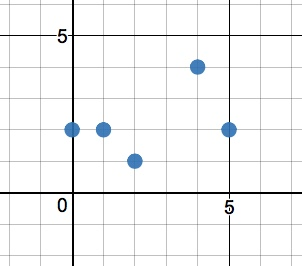
\includegraphics[width=0.25\textwidth]{discrete-domain-graph.jpeg}
\end{figure}

\item What is the range of the given function modeling a bicycle wheel?

\begin{figure}[!ht]
    \centering
    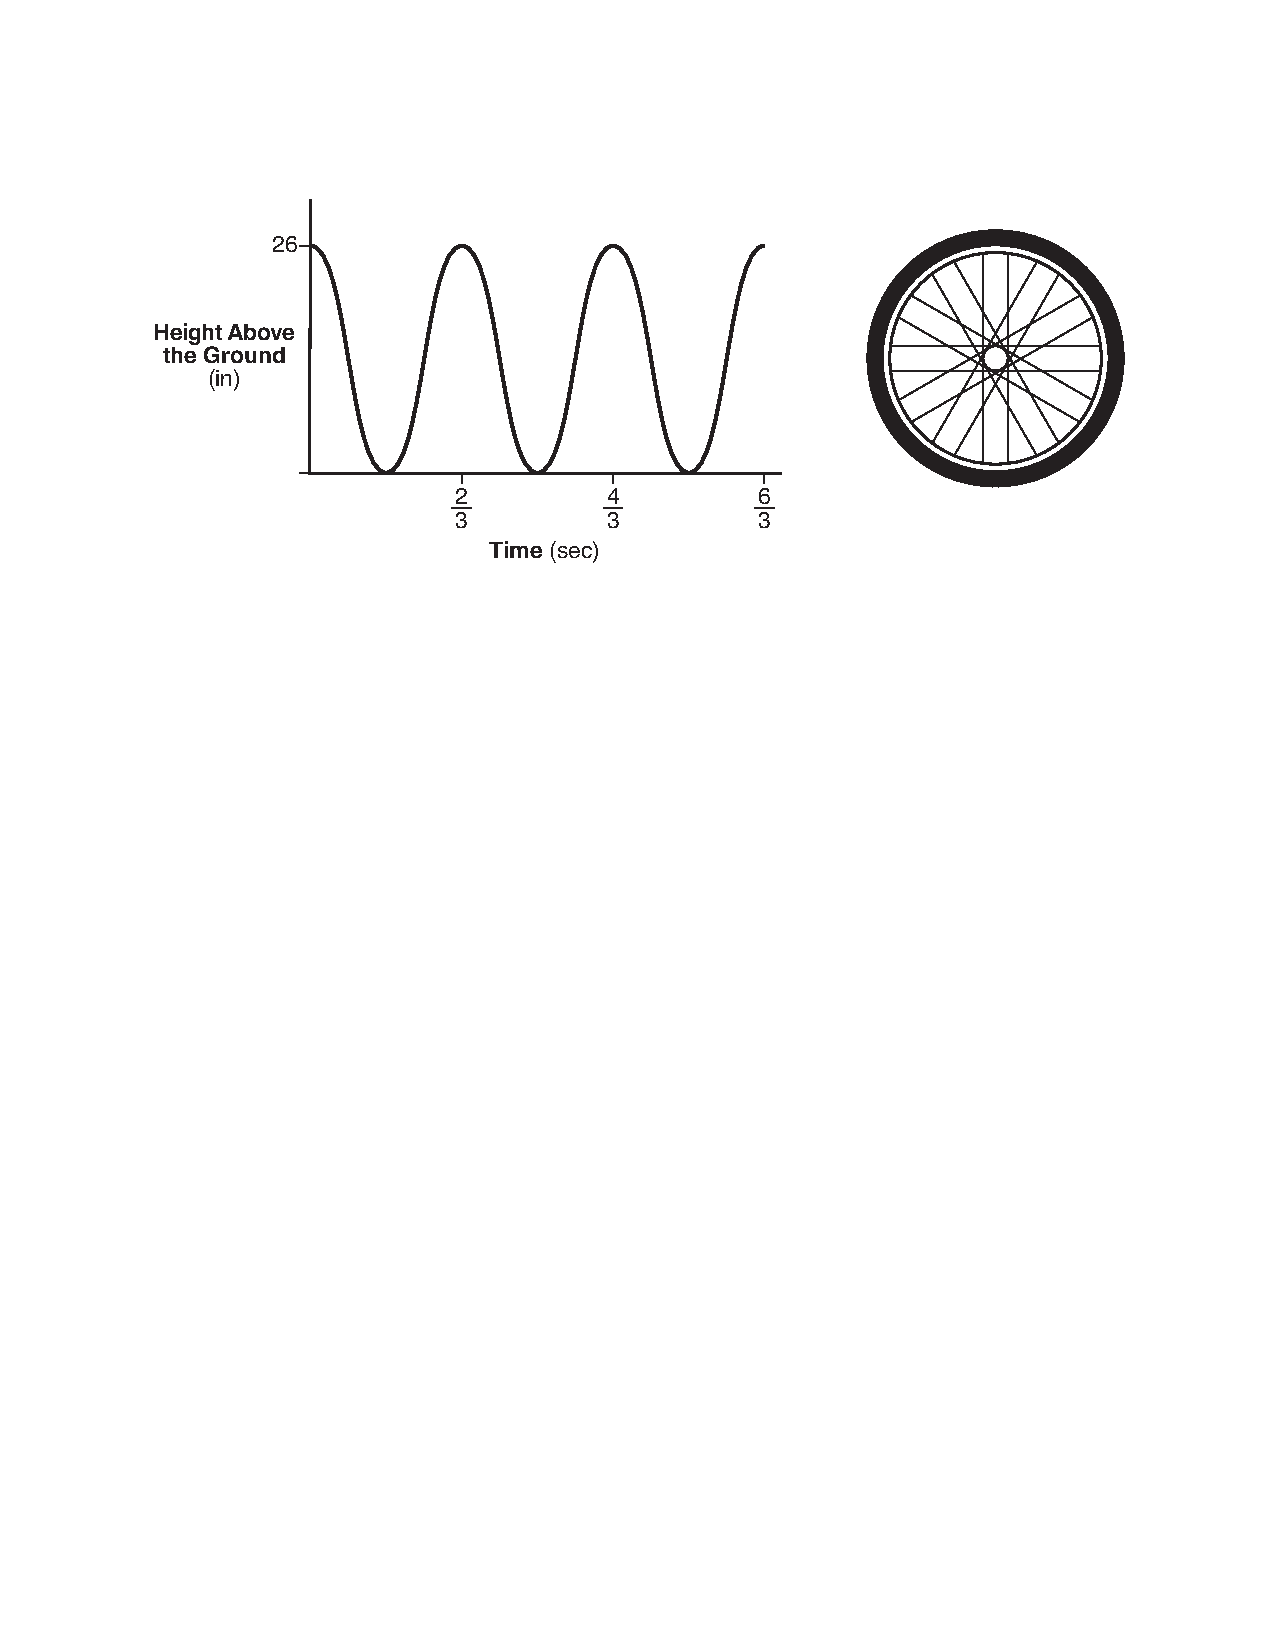
\includegraphics[width=0.65\textwidth]{sine-bike-wheel.pdf}
\end{figure}

\subsection*{Function transformations}
Describe how the functions below have transformed from the parent function $f(x)=|x|$.
\item $g(x)=|x+2|$
\item $h(x)=-|x|+2$

\newpage

\subsection*{Sketching a quadratic function}
Answer in the space provided. (you may also use additional lined paper)
\item   Given $f(x)=-(x-3)^2+16$
\begin{enumerate}
    \item Write down the vertex of the function as an ordered pair.\\*[10pt]
    \item Write down the equation of the axis of symmetry.\\*[10pt]
    \item Expand the function from vertex form to standard form, $ax^2+bx+c \text{ where } a, b, c \;  \epsilon \; \mathbb{R}$.\\*[20pt]
    \item Write down the value of $f(0)$. Explain what this represents on the graph.\\*[10pt]
    \item Hence factor the function. Write down the roots.\\*[20pt]
    \item Sketch the function, labeling the intercepts with values and the vertex as an ordered pair. Show the axis of symmetry as a dotted line and label it with its equation.
\begin{figure}[!ht]
    \flushright
    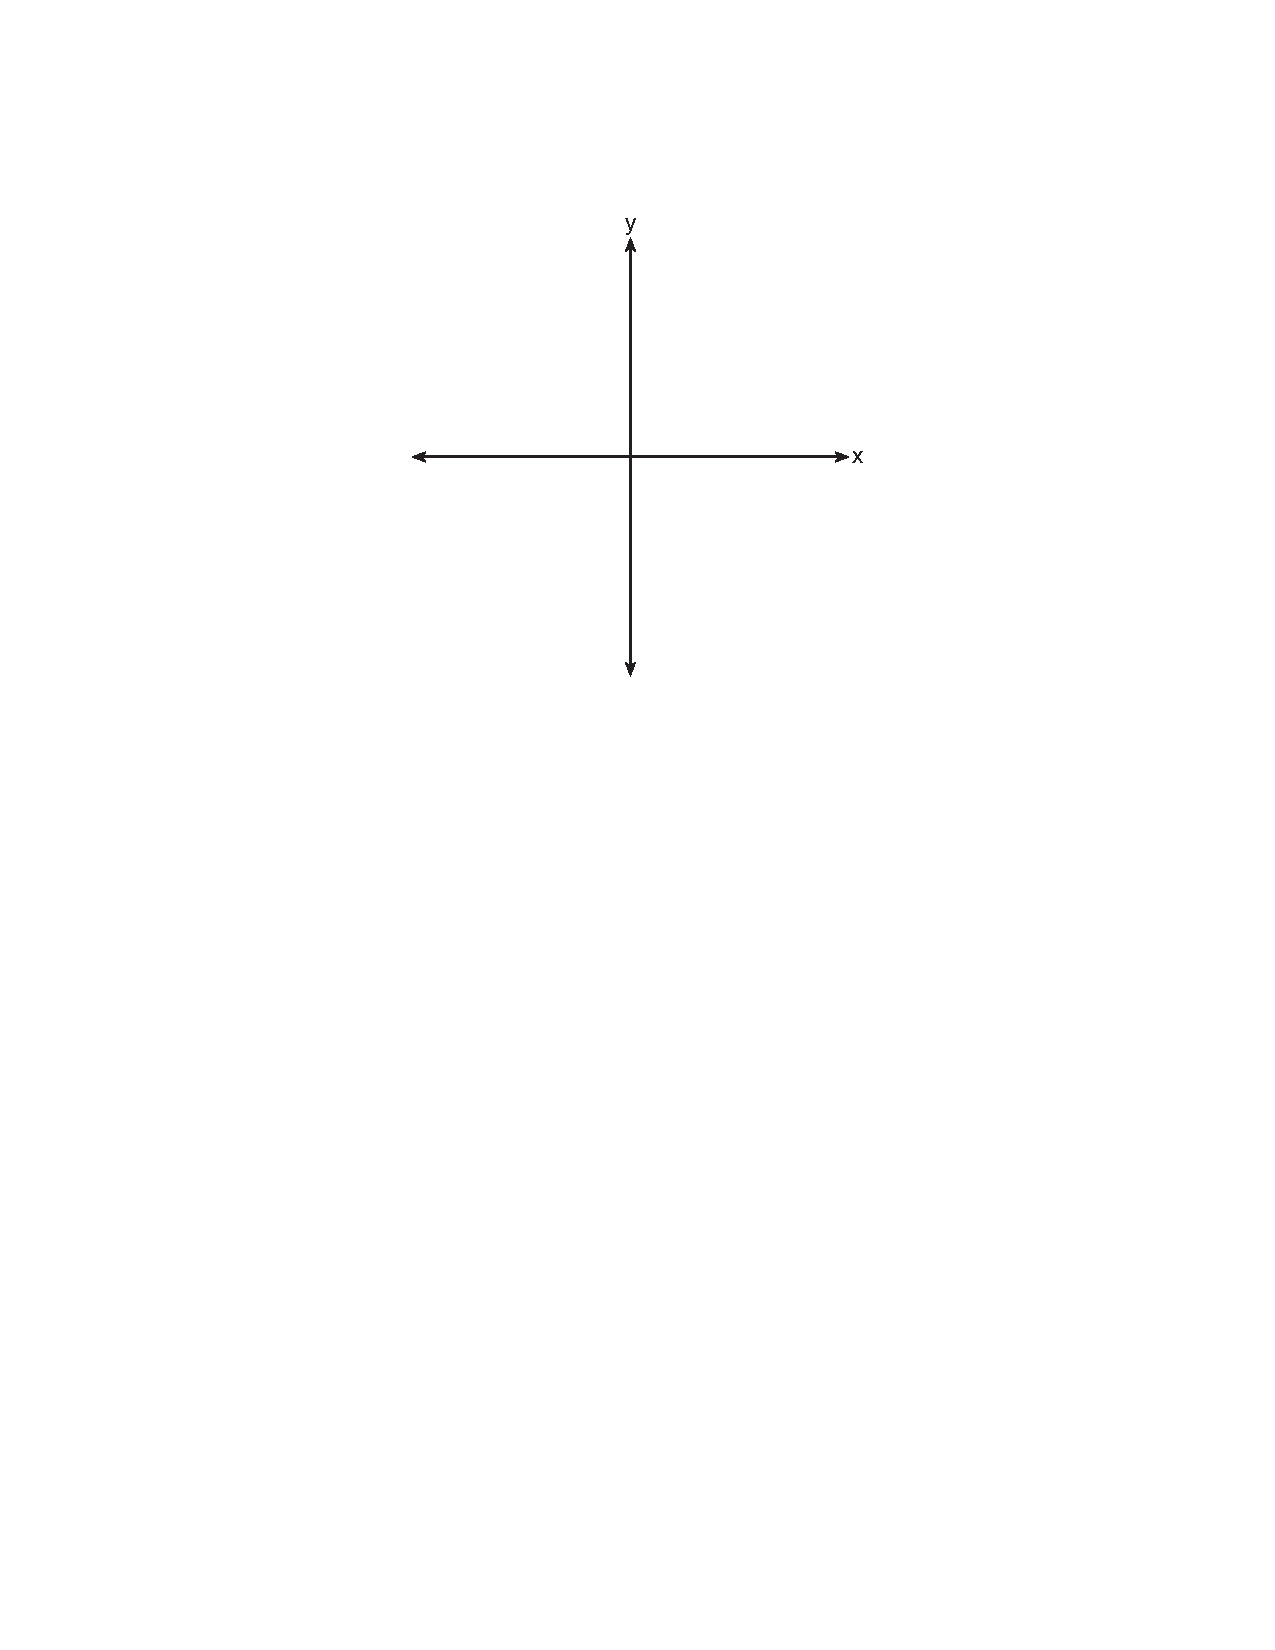
\includegraphics[width=0.6\textwidth]{simple-axes.pdf}
\end{figure}

    \item Write down the domain and range of the function.\\*[10pt]
\end{enumerate}


\newpage
\subsection*{Graphing quadratics}
Answer on lined paper. Graph the function on the grid shown below.
\item Given the function $f(x)=-x^2-x+6$. 
\begin{enumerate}
    \item Write down the $y$-intercept.
    \item State whether the parabola opens upward or downward. Explain how you know this from the function expressed in standard form.
    \item Express the function in factored form. Hence state the solutions to $f(x)=0$.
    \item Show that the axis of symmetry of the parabola is $x=-\frac{1}{2}$.
    \item Hence state the vertex as an ordered pair. 
    \item Graph the function. Mark the vertex as an ordered pair and label each intercept with its value. Plot the axis of symmetry as a dotted line and label it with its equation.
    \item Write down the domain and range of the function.
\end{enumerate}

\begin{figure}[!ht]
    \centering
    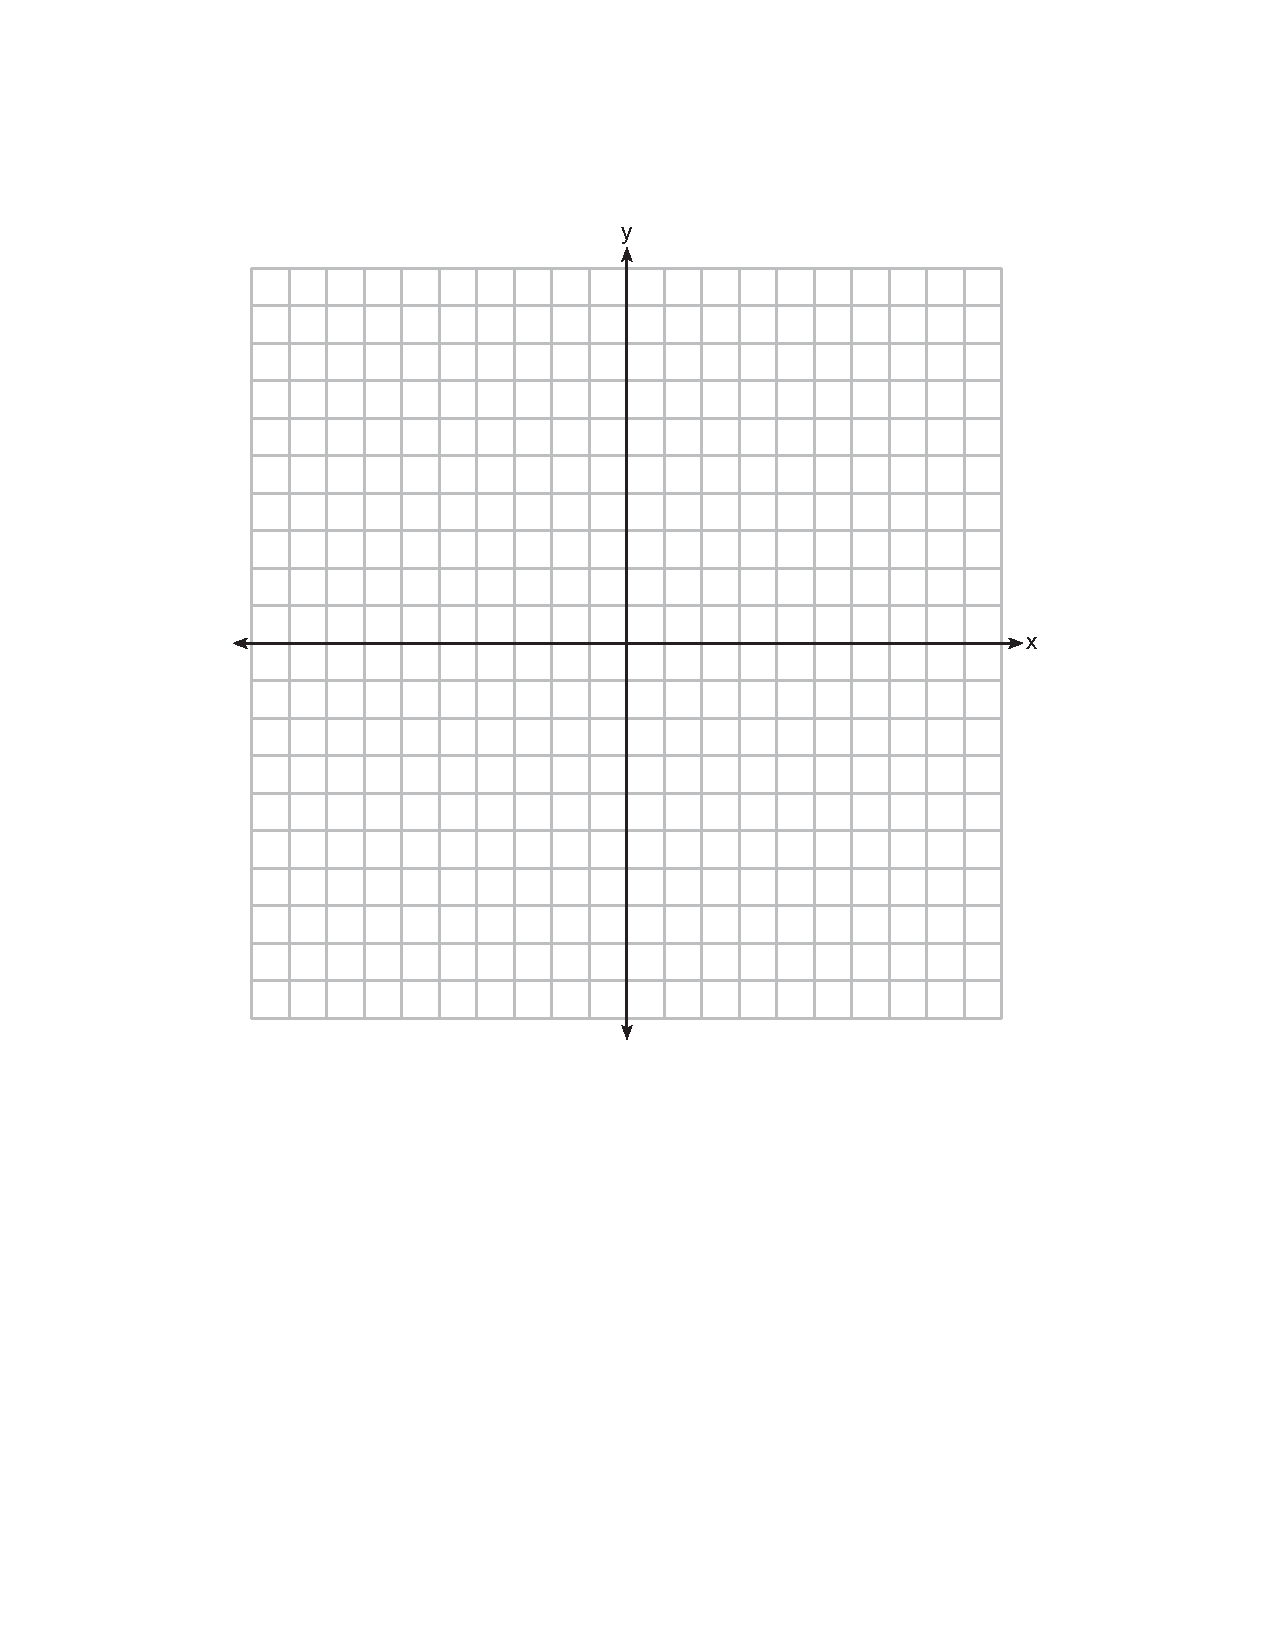
\includegraphics[width=0.75\textwidth]{regents-grid.pdf}
\end{figure}

\newpage
\item  
\begin{enumerate}
    \item Graph the parent function $f(x)=x^2$. Mark the point $P(3, f(3))$ on the graph
    \item The function $g(x)$ is the function $f$ after being translated to the right 5 and down 4. Graph $g$.
    \item Mark the point on the function $g$, $Q$, that represents the point $P$ after the translation.
\end{enumerate}

\begin{figure}[!ht]
    \centering
    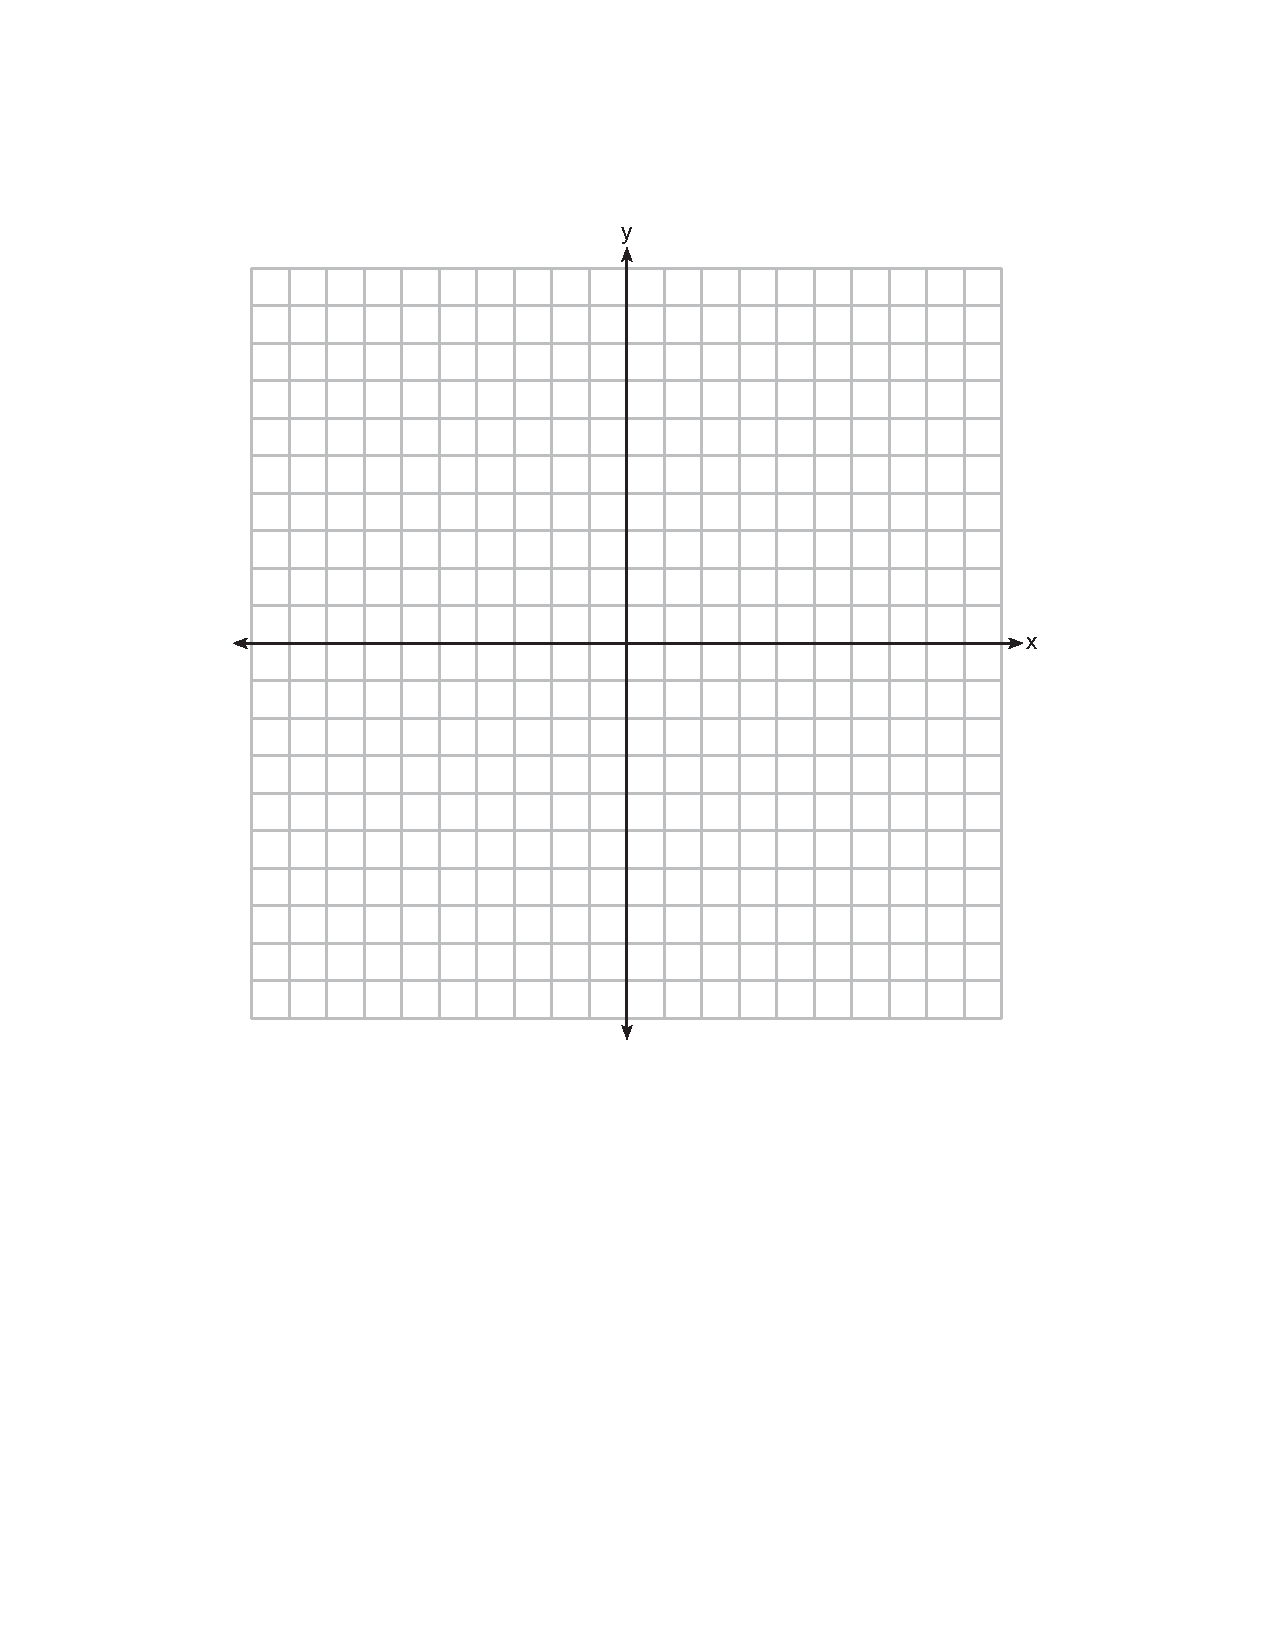
\includegraphics[width=0.75\textwidth]{regents-grid.pdf}
\end{figure}

\newpage
\subsection*{Model situations with quadratic functions}
\item The path of a diver is given by 
\[f(x)=-5x^2+12x+9\]
where $y$ is the height (in meters) and $x$ is time in seconds.\\*[5pt]
\begin{enumerate}
    \item On the grid below, graph the function over the domain where $x\geq 0$ and the range where $f(x) \geq 0$. Use a horizontal scale of 5 squares equals one second and vertical scale of 1 square equals one meter. Label the intercepts and vertex.
    \item What is the maximum height of the diver? Label the point on the graph with the work ``max.''\\*[30pt]
    \item What is the time when the diver enters the water? Label the point on the graph representing this with the word ``splash.''\\*[30pt]
\end{enumerate}

\begin{figure}[!ht]
    \flushright
    
\includegraphics[width=0.65\textwidth]{1stQ-grid.pdf}
\end{figure}

\subsection*{Honor pledge}
I have not received human help with this test, nor have I used calculators (including Desmos) except for an approved graphing calculator. Signed:

\end{enumerate}
\end{document}